% Chapter X

\chapter{Onderzoek: SOUP analyse}\label{ch:onderzoek:-soup-analyse} % Chapter title

\begin{itemize}
\item https://jeremylong.github.io/DependencyCheck/
\end{itemize}

Voordat we verder kijken naar mogelijkheden om kwetsbaarheden in een externe bibliotheek te onderzoeken en te verhelpen moeten we eerst kijken naar een aantal kernbegrippen om te begrijpen waar het om gaat.

Dit onderzoek heeft daarom ook twee hoofdvragen die ieders weer een aantal deelvragen opwerpen.
Als eeste is de vraag "Welke kwetsbaarheden bestaan er hoe is het gebruik van externe bibliotheken hier aan gecorreleerd?
De deelvragen die hier uit voorkomen luiden:
\begin{itemize}
  \item Wat zijn applicatie veiligheidsrisico's?
  \item Welke komen het meest voor?
  \item
\end{itemize}

\section{Wat zijn applicatie veiligheidsrisico's}\label{sec:wat-zijn-applicatie-veiligheids-risico's}
Veiligheids risico's binnen applicaties zijn een som van kwetsbaarheden die zich bedoeld of onbedoeld in de applicatie bevinden, de vindbaarheid en de "schade" die er mee aangericht kunnen worden.
De termen van de som worden hieronder verder uitgediept als ook een top-10 uitgeven door de OWASP van de meest voorkomende kwetbaarheden.

Een aanvaller kan op meerdere manier in een applicatie komen(figuur X).
Vaak gebeurt dit door een kwetsbaarheid van een applicatie te zoeken en deze te exploiteren.
Als er vervolgens geen maatregeling genomen zijn om de aanvaller te weerhouden kunnen er zaken als data in een database, assets van het bedrijf of zelfs functionaliteit aangetast worden.
Wat op zijn beurt weer voor een impact in de bedrijfsvoering kan veroorzaken.
Hoe aanvallers een applicatie kunnen aanvallen is applicatie specifiek
De impact op de bedrijfsvoering is ook specifiek
\begin{figure}[H]
  \myfloatalign
  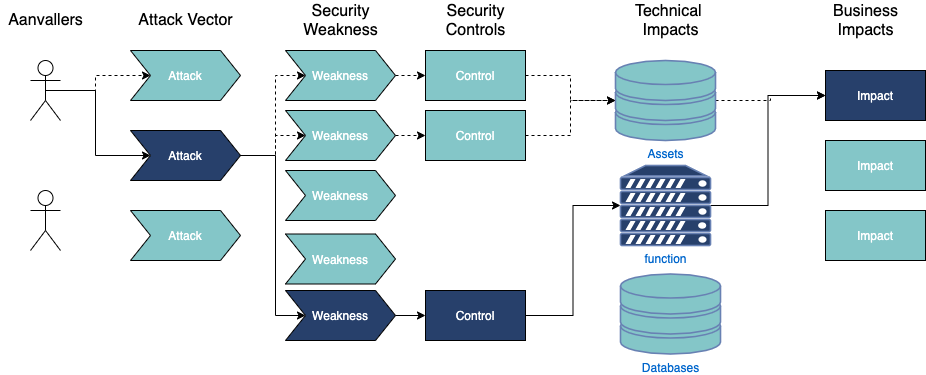
\includegraphics[width=15cm]{gfx/application security routes}
  \caption{Aanvalllen, en hun gevolg}
  \label{fig:Application Security Routes}
\end{figure}

Veiligheids risico's kunnen in categoriën worden geplaatst middels een gradatie systeem die in figuur x te ze zien is.
De OWASP-Top10 die verder in de tekst te vinden is maakt gebruik van dit gradatie systeem om risico's in te schalen.
OWASP is een instantie die zich bezighouden met het verbeteren van de veiligheid van applicaties.
Het doet dit door onder andere training en erkenning te geven aan kwetsbaarheden.
Zo wordt er eens in de 5 jaar een top-10 samengesteld met de op dat moment meest voorkomende kwetsbaarheden.
\footnote{Helaas is de laatste versie die aan het einde van 2021 uit moet komen nog niet beschikbaar op het moment van schrijven}
De OWASP-Top10 wordt samengesteld uit data van meer dan 100.000 productie applicaties en APIs wat door meer dan 500 mensen is getest door 40 verschillende bedrijven.
De top 10 is een aggegratie van deze data in de meest voorkomende issues met inachtneming van exploitabity, detectability en impact.


\begin{figure}[H]
  \myfloatalign
  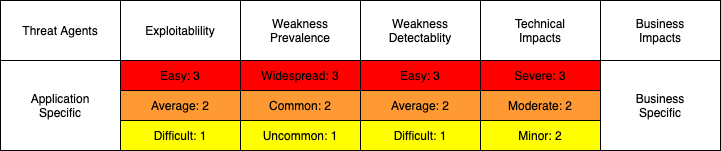
\includegraphics[width=12cm]{gfx/risk tabel}
  \caption{Inschaling van risico's}
  \label{fig:risico inschaling}
\end{figure}

%threat agents = aanvallende entiteit
%exploitabity = exploiteetbaatheid
%weakness prevalance = vookomendheid van de zwakte in een applicatie
%weakness detectability = hoe goed is de zwakte in een applicatie te detecteren
%technical impact = technische impact op de applicaties
%business impacts = (zakelijke impact) impact op de bedrijfsvoering

\begin{itemize}

%Bron: https://codebros.nl/blog/wat-is-de-owasp-top-10 , https://owasp.org/www-project-top-ten/ << PDF download

  \item \textbf{A01:2017 Injection [exploitabity: 3, Prevelance: 2, detectability: 3, technical: 3] :} \\
  De mogelijkheid om OS, SQL, NoSQL commandos te injecteren in web applicaties zorgt ervoor dat aanvallers toegang kunnen hebben tot delen van systemen zonder er recht op te hebben.\ Daarnaast is er ook de mogelijkheid om toegang te krijgen tot data die niet voor hen bedoelt is.

  \item \textbf{A02:2017 Broken Authentication [exploitabity: 3, Prevelance: 2, detectability: 2, technical: 3]:}\\ Het verkeerd implementeren van authentication en session management kan er voor zorgen dat aanvallers wachtwoorden, sessie tokens aan kunnen passen om zo zich voor te doen als een andere gebruiker.

  \item \textbf{A03:2017 Sensitive Data Exposure [exploitabity: 2, Prevelance: 3, detectability: 2, technical: 3]:}\\
  Het verkeerd of niet voldoende afschermen van APIs kunnen ervoor zorgen dat sensitive data makkelijk gevonden kan worden.\ Zeker als de data niet encrypted verzonden wordt.

  \item \textbf{A04:2017 XML External Entities (XXE) [exploitabity: 2, Prevelance: 2, detectability: 3, technical: 3]:}\\
  Veel oude of slecht geconfigureerde XML-processoren evalueren externe entiteit referenties binnen XML documenten slecht. Hierdoor is het mogelijk om links te cree\"en naar bestanden en/of fileshares waar code staat die slecht is voor de applicatie [that contains malicious code].

  \item \textbf{A05:2017 Broken Access Control [exploitabity: 2, Prevelance: 2, detectability: 2, technical: 3]:}\\
  Restricties op wat een geauthenticeerde gebruikers mogen worden niet altijd nageleefd, Aanvallers kunnend deze fouten gebruiken om toegang te krijgen tot gegevens of functionaliteiten die niet bestemd zijn voor deze gebruikers. Ze kunnen gegevens aanpassen en of toegangsrechten aanpassen.

  \item \textbf{A06:2017 Security Misconfiguration [exploitabity: 3, Prevelance: 3, detectability: 3, technical: 2]:}\\
  Slechte configuratie van de veiligheids instellingen zijn de meest gevonden ??issue??. Dit is meestal het gevolg van het gebruiken van de default, incomplete of ad-hoc configuratie Hierdoor kunnen cloud storages open komen te staan, verkeerd geconfigureerde HTTP headers of foutmeldingen die te veel informatie meegeven ontstaan.

  \item \textbf{A07:2017 Cross-Site Scripting (XSS) [exploitabity: 3, Prevelance: 3, detectability: 3, technical: 2]:}\\ middels XSS is het mogelijk om scripts te draaien van een andere bron dan wenselijk. Dit geeft de mogelijkheid om via een browser andere scripts in de applicatie te draaien zo proberen andere functionaliteiten toe te voegen. Wat kan resulteren in een web site dat zich anders gedraagt dan de bedoeling is.

  \item \textbf{A08:2017 Insecure Deserialization [exploitabity: 1, Prevelance: 2, detectability: 2, technical: 3]:}\\ Door het niet veilig serialiseren van objecten naar text kan het voorkomen dat er code of commando's mee worden gestuurd welke uitgevoers kunnen worden op de server.

  \item \textbf{A09:2017 Using components with Known vulnerabilities [exploitabity: 2, Prevelance: 3, detectability: 2, technical: 2]:}\\
  Componenten zoals bibliotheken, frameworks en andere software modules die gebruikt worden voor het ontwikkelen van een applicatie kunnen bedoelt en of onbedoeld [malicious code ] bevatten Wat kan resulteren in verschillende mogelijkheden voor de aanvaller binnen te dringen. of data te versturen naar een andere host om zo achter "beveiligde" gegevens te komen.

  \item \textbf{A10:2017 Insuffivient Logging \& Monitoring[exploitabity: 2, Prevelance: 3, detectability: 1, technical: 2]:}\\
  Logging en monitoring is bijna net zo belangrijk als het ontwikkelen van een veilige applicatie, mocht er toch een aanval plaatsvinden op welke manier dient er de mogelijkheid zijn om terug te zien wat er precies gebeurt is. Logging zorgt hiervoor. Het monitoring deel is het bekijken van de logs om te zien of er iets verdachts plaats heeft gevonden. Er zijn tools beschikbaar die er voor automatische monitoring zorgen( Nagios is dit soort tool)

\end{itemize}


In het vorige hoofdstuk is te lezen dat Eaglescience gebruik maakt van de volgende technologi\"en: Scala 2.XX, TypeScript, Jenkins, Docker ,Azure cloud.

Dit onderzoek richt voornamelijk op kwetbaarheden in bibliotheken  van derden en de bestrijding ervan.
En specifiek op de bovenstaande door Eaglescience gebruikte technieken.
De hoofdvraag voor dit hoofdstuk luid dan ook: "Met welke kwetsbaarheden hebben we te maken binnen Eaglescience en hoe kunnen we deze opsporen op een automatiseerde manier zonder de huidige werkwijze te verstoren?" Uit deze hoofdvraag onstaan de volgende deelvragen die in dit onderzoek beantwoord worden met daarna een conclusie op de hoofdvraag.

\begin{itemize}
\item Welke soorten kwetsbaarheden zijn er?
\item Hoe kunnen deze kwetbaarheden hun weg vinden in onze gebouwde software?
\item Zijn er instanties die bijhouden waar zich kwetsbaarheden schuilhouden?
\item Wat zijn methodes om te onderzoeken of er in de bestaande software kwetbaarheden bevinden?
\item Is er een mogelijkheid om een third-party pakket in te zetten om dit te doen?
\end{itemize}

\

Binnen Eaglescience wordt er heel goed gekeken naar de manier waarop er veilige software ontwikkeld wordt.
Zaken die in de OWASP top-10 staan wordt serieus mee omgegaan en actief tegen gehandeld. zo wordt er ook gegekeken naar het gebruik van bibliotheken van derden.

Op plaats A09:2017 is te vinden dat er kwetsbaarheden middels bibliotheken van derden binnen kunnen komen. Dit is iets wat deels buiten het bereik van Eaglescience ligt. Om ons hier tegen te beschermen is het wenselijk om periodiek en geautomatiseerd een analyse naar kwetbaarheden tedoen.

De bibliotheken die gebruikt worden van derden wordt ook wel Software of unkown pedigree genoemd of kortweg SOUP. Dit houdt in dat een bibliotheek wordt ontwikkeld middels een proces of methode wat niet bekend is bij de eindgebruiker. Ook zijn vaak de details niet bekend van de bibliotheek omdat deze niet of nauwelijks wordt gereviewed door de eindgebruiker. Om deze reden is het dus onbekend of er kwetsbaarheden zitten in betreffende bibliotheken.
De definitie van SOUP blijft niet alleen bij de bibliotheken en frameworks vanuit het open-source gebied. Veelal is ook niet bekend hoe closed-source (Proprietary software) wordt geschreven, echter door reputatie van bedrijven die deze software schrijven wordt veelal , onterecht\footnote{zie: https://www.nu.nl/tech/6097701/waarom-de-hack-bij-solarwinds-ministeries-en-grote-bedrijven-treft.html } aangenomen dat deze geen lekken bevatten.

\section{CVE}
in de appliction security wordt er gesproken van een CVE(Common Vulnerability en Exposures) als een kewtsbaarheid bekend is deze wordt in een database geplaatst zodat \'e\'en ieder die geintreseerd is hier kan vinden welke software(os, applicatie, framework, bibliotheek) mogelijk niet veilig is. Deze Database wordt in stand en bijgehouden door een aantal instanties waarbij de belangrijksten zijn:
\begin{itemize}
  \item \textbf{NIST-CSRC} Computer Security Research Center van het National Institute of Standards and Technology) is een centrum dat onderzoek doet namens de Amerikaanse regering naar veiligheden in software. De database die het NIST-CSRC bijhoud heet het NVD(National Vulnerability Database) waarin CVE's worden bijgehouden.
  \item \textbf{CVE-Mitre} is een community driven effort wat CVE's logt in een lijst die vervolgens de NVD voedt met hun gevondendata.
  \item \textbf{cvedetails.com/}
  \item \textbf{vuldb.com/}
  \item \textbf{https://www.exploit-db.com/}
\end{itemize}

\section{}

https://www.security.nl/posting/666663/Van+CVE+tot+CVSS\%3A+wegwijs+in+het+woud+van+kwetsbaarheden










\section{Zijn er instanties die bijhouden waar zich kwetsbaarheden schuilhouden?}

Naast OWASP zijn er nog een aantal instanties dit bijhouden welke software\footnote{zoals hier gebruikt in de bereedste? zin van het woord dus: (Operating systems, ontwikkeltalen/databases, ontwikkelframeworks,bibliotheken) }
mogelijk kwetsbaarheden kunnen bevatten.
\begin{itemize}

\end{itemize}


\section{Wat zijn methodes om te onderzoeken of er in de bestaande software kwetbaarheden bevinden?}

\section{Is er een mogelijkheid om een third-party pakket in te zetten om dit te doen?}
